In this section we are supposed to explain the behaviour of the value of the contract with for three different values of $r$. Firstly, let's plot out a graph in which we can see the behaviour of the value of the option as $S$ increases, as we are told to do. This can be found in Figure \ref{analysisDifferent_r_withoutZoom}. However, we do not see a great different between the three lines: only in $S\in[10,30]$ seems to be a different behaviour, exactly within the region where the contract is held. Hence, in order to provide a better analysis about the behaviour of this contract with the different $r\in\{0.0058,0.0117,0.0175\}$, we have plotted the value of the contract when $S\in[18,24]$. We can see that the value increases as $r$ decreases. This can be explained by looking at (\ref{useful}): the three values of the contract are given by a fraction in which the numerator is common among all of them and the denominator consists of a product of $r$ with a constant. Hence, it's obvious that as $r$ decreases, then the value of the contract increases.

On the other hand, the $r$ only appears one time in all the formul\ae \ (where we have described). Therefore, the contribution of a slight change in $r$ will provide also a slight change in $V$.
\begin{figure}[h]
	\centering
	\begin{subfigure}[t]{0.5\textwidth}
		\centering
		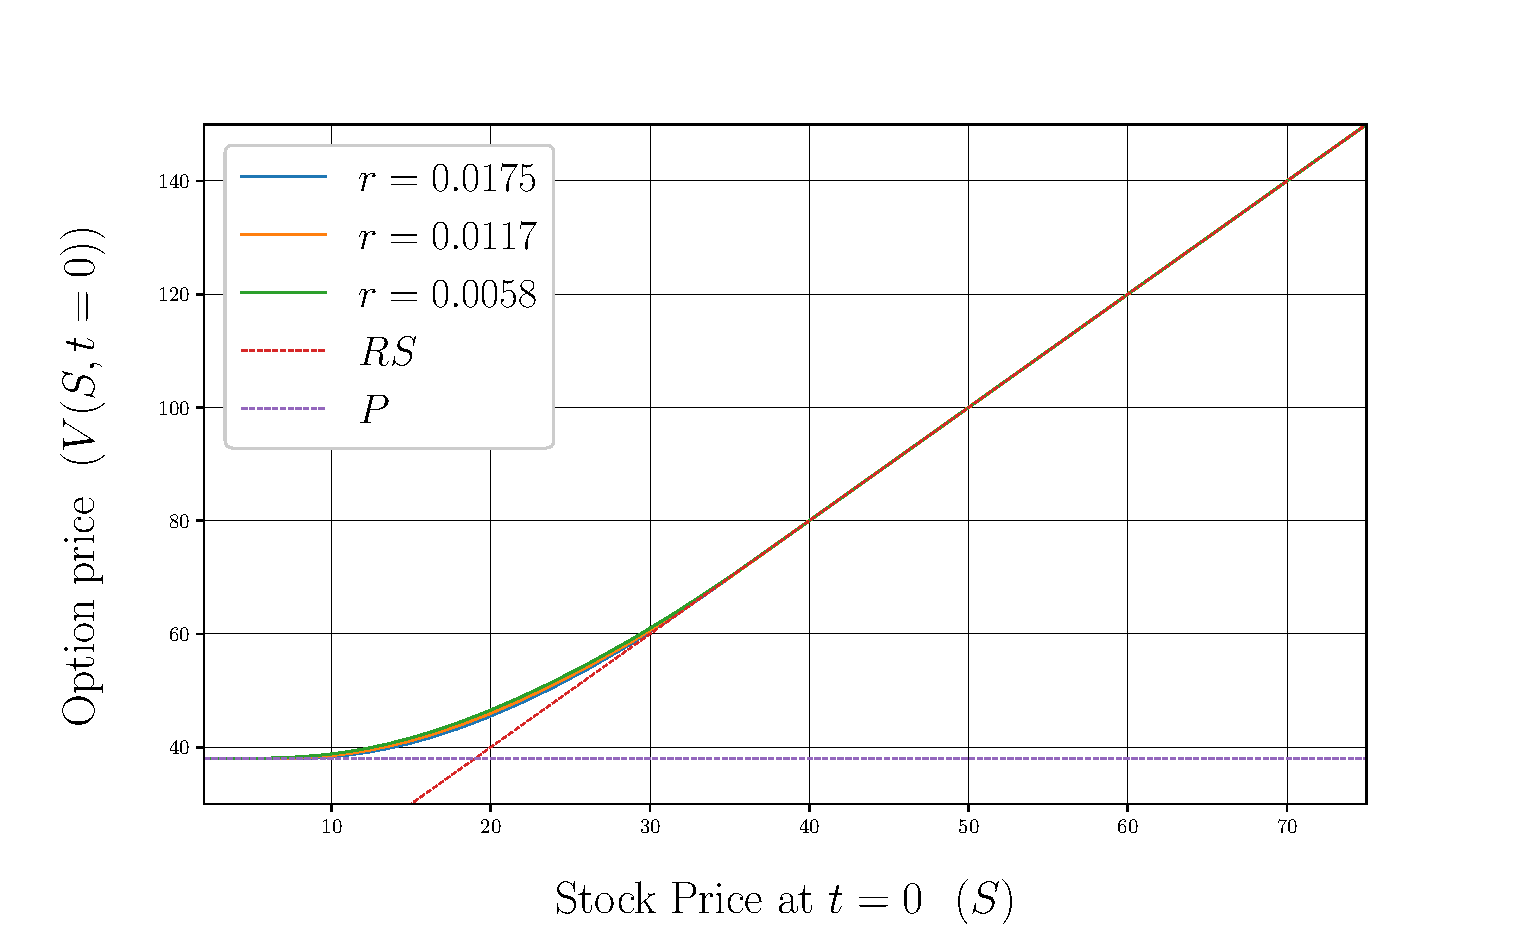
\includegraphics[scale=0.36]{img/Q2/amConvBondValues_incrS_DifferentInterestRates}
		\captionsetup{width=0.65\linewidth, font=footnotesize}
		\caption{Without zoom.}\label{analysisDifferent_r_withoutZoom}
	\end{subfigure}%
	\begin{subfigure}[t]{0.5\textwidth}
		\centering
		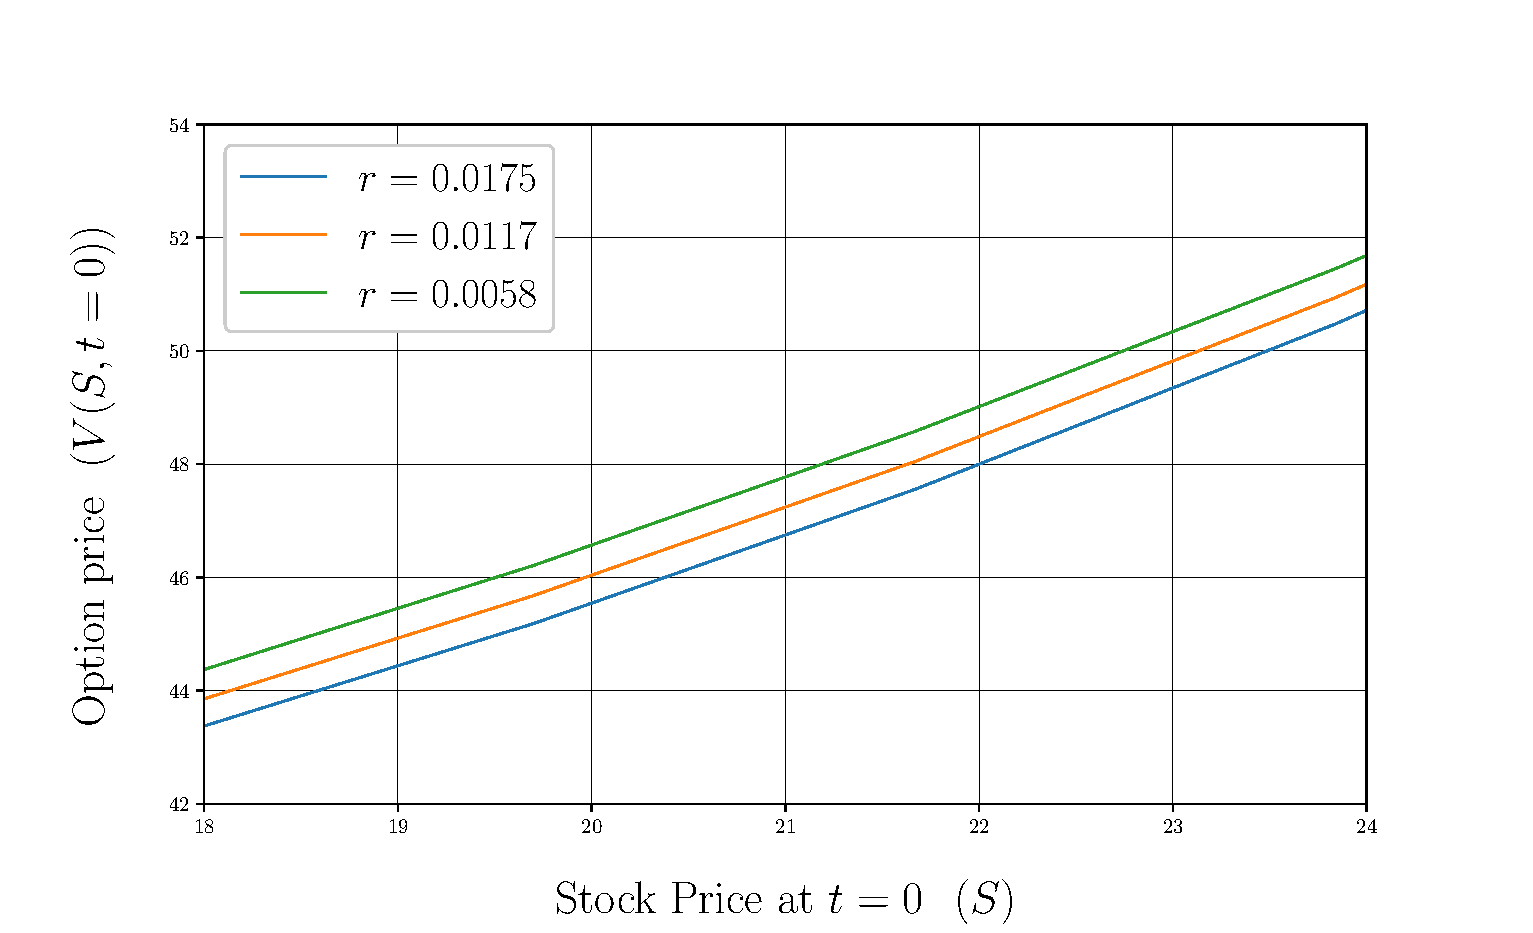
\includegraphics[scale=0.36]{img/Q2/amConvBondValues_incrS_DifferentInterestRatesZoom}
		\captionsetup{width=0.65\linewidth,font=footnotesize}
		\caption{Zoom on $V(S,0)\in [18,24]$.}\label{analysis_different_r_Zoom}
	\end{subfigure}
	\caption{Value of the contract with $r\in\{0.0058,0.0117,0.0175\}$ as $S$ increases.}\label{analysisDifferent_r}
\end{figure}
